\scanpage{136}
\diagram{\begin{tikzcd}[ampersand replacement=\&,column sep=large,row sep=large]
 \& \mathrm{Pro}(\mathrm{Sch}/S) \arrow[d,phantom,"\cup"{description},"{\substack{\text{sous-catégorie}\\\text{pleine}}}"{anchor=west,xshift=8pt}] \& \text{pro-préschémas}\\
(\mathrm{Sch}/S) \& \mathrm{Pro}'(\mathrm{Sch}/S) \arrow[l,"\varprojlim"'] \arrow[d,phantom,"\cup"{description},"{\substack{\text{sous-catégorie}\\\text{pleine}}}"{anchor=west,xshift=8pt}] \& \text{pro-préschémas }(X_i)_{i\in I},\ \text{t.q. }\exists i,\ \unsure{u_{ji}|\varphi_{ij}}\ \text{affines pour }j\geq i\\
 \& \mathrm{Pro}''(\mathrm{Sch}/S) \arrow[ul,"{\substack{\text{foncteur}\\\text{pleinement}\\\text{fidèle}}}"{anchor=north east,xshift=-5pt,yshift=-3pt}] \& \text{pro-préschémas }(X_i)_{i\in I}\ \text{t.q.}
\end{tikzcd}}
\deleted{\[\left\{\begin{array}{l}\unsure{X_i\ \text{quasi-cpt. et de présentation finie}}\\ \exists i,\ [\unsure{u_{ji}|\varphi_{ij}}\ \text{affines de prés. }\unsure{\text{finie}}]\end{array}\right.\]}
\[
\left\{\begin{array}{l}
\forall i\,\unsure{\mathrm{gd}|\mathrm{quel}},\ X_i\ \text{est qu. cpt et de présentation finie sur }S\\
\exists i\ \text{t.q. }j\geq i\ \text{implique }\unsure{u_{ji}|\varphi_{ij}}\ \text{affine.}
\end{array}\right.
\]

Soient $\unsure{\mathcal X|\mathfrak X}\in\mathrm{Ob}\,\mathrm{Pro}''(\mathrm{Sch}/S)$, $\mathcal Y\in\mathrm{Ob}\,\mathrm{Pro}'(\mathrm{Sch}/S)$ \inserted{$\mathcal Y=(Y_j)$, les $Y_j$ quasicompacts}, alors
\[
\mathrm{Hom}_{\mathrm{Pro}(\mathrm{Sch}/S)}(\mathcal Y,\unsure{\mathcal X|\mathfrak X})\overset{\sim}{\longrightarrow}\mathrm{Hom}(\varprojlim\mathcal Y,\varprojlim\unsure{\mathcal X|\mathfrak X})
\]
\deleted{[En particulier, la catégorie}
\inserted{Si on est sur une base $S$}
\[
\mathrm{Hom}_{\mathrm{Pro}(\mathrm{Sch}/S)}(\mathcal Y,\unsure{\mathcal X|\mathfrak X})\overset{\sim}{\longrightarrow}\mathrm{Hom}_S(\varprojlim\mathcal Y,\varprojlim\unsure{\mathcal X|\mathfrak X})
\]

\deleted{Dans les provariétés de Serre}

\uline{Remarque} Dans Serre et Néron, on utilise des systèmes projectifs de schémas \inserted{(algébriques)} qui sont \inserted{(pratiquement tjs)} $\in\mathrm{Pro}''(\mathrm{Sch})$.
\deleted{\unsure{Donc}} Il y a avantage à les ``interpréter'' comme étant de véritables schémas sur $k$, \unsure{et non bien|et non rien} des pro-objets $\ldots\ldots$.
\figure{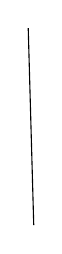
\begin{tikzpicture}\draw (0,0)--(-.07,2.5);\end{tikzpicture}}
\margin{135}
